\subsection{IllustrisTNG}
IllustrisTNG \footnote{https://www.tng-project.org/} is the follow-up project after the success of the Illustris simulations \parencite{Springel2017, Pillepich2017,Naiman2018, Nelson2017, Marinacci2018}. It is a huge project, built upon a magneto-hydrodynamical cosmological simulation code with added physical processes on a subgrid level \parencite{Weinberger2016}. Adding physical processes like gas radiation, star formation, stellar feedback through supernova explosions, supermassive black hole accretion and magnetic fields is essential to model galaxy formation and evolution and allows for a much better comparison to reality compared to dark matter-only simulations. The data output from the simulations is extensive, and is not meant to be analyzed all in one go, but rather through a series of analyzes, each targeting a specific scientific question. 


\subsubsection{The simulations}
The IllustrisTNG project includes 18 different simulations with varying resolutions, spatial size, and included physics. There are three main simulations, TNG300, TNG100, and TNG50, that differ in volume and resolution. The details of these are summed up in Table \ref{TNG}. Each of the main simulations has been run at three different resolution levels, which makes it possible to study how the outcome is affected by changing only the resolution in a given simulation. TNG100 has a physical box volume of $110.7^3 \, $Mpc$^3$, and a baryonic particle resolution of $1.4 \times 10^6 M_{\odot}$, while the TNG300 simulation has a volume of $302.6^3 \, $Mpc$^3$ and a baryonic particle resolution of $1.1 \times 10^7 M_{\odot}$. The newly released third simulation, TNG50, has a smaller volume of $51.7^3 \, $Mpc$^3$, but with a much higher baryonic particle resolution of $8.5 \times 10^4 M_{\odot}$. 

In this project, a large statistical sample of galaxies was needed, as well as a resolved structure of the inner part of the galaxies to calculate the different properties, so the TNG100 simulation was the best choice with respect to size and resolution. The TNG100-1 simulation data, which is the highest available resolution for TNG100, has been used throughout the project and will from now on be referred to as TNG only. A visual representation of parts of the simulations can be seen in Figure \ref{tng_illustration}. For its cosmology parameters TNG uses the results from the Planck Collaboration, which are given by $\Omega_{\Lambda,0} = 0.6911$, $\Omega_{m,0}=0.3089$, $\Omega_{b,0}=0.0486$, $\sigma_8=0.8159$, $n_s=0.9667$ and $h = 0.6774$ \parencite{Planck2016}.

\begin{figure}
    \centering
    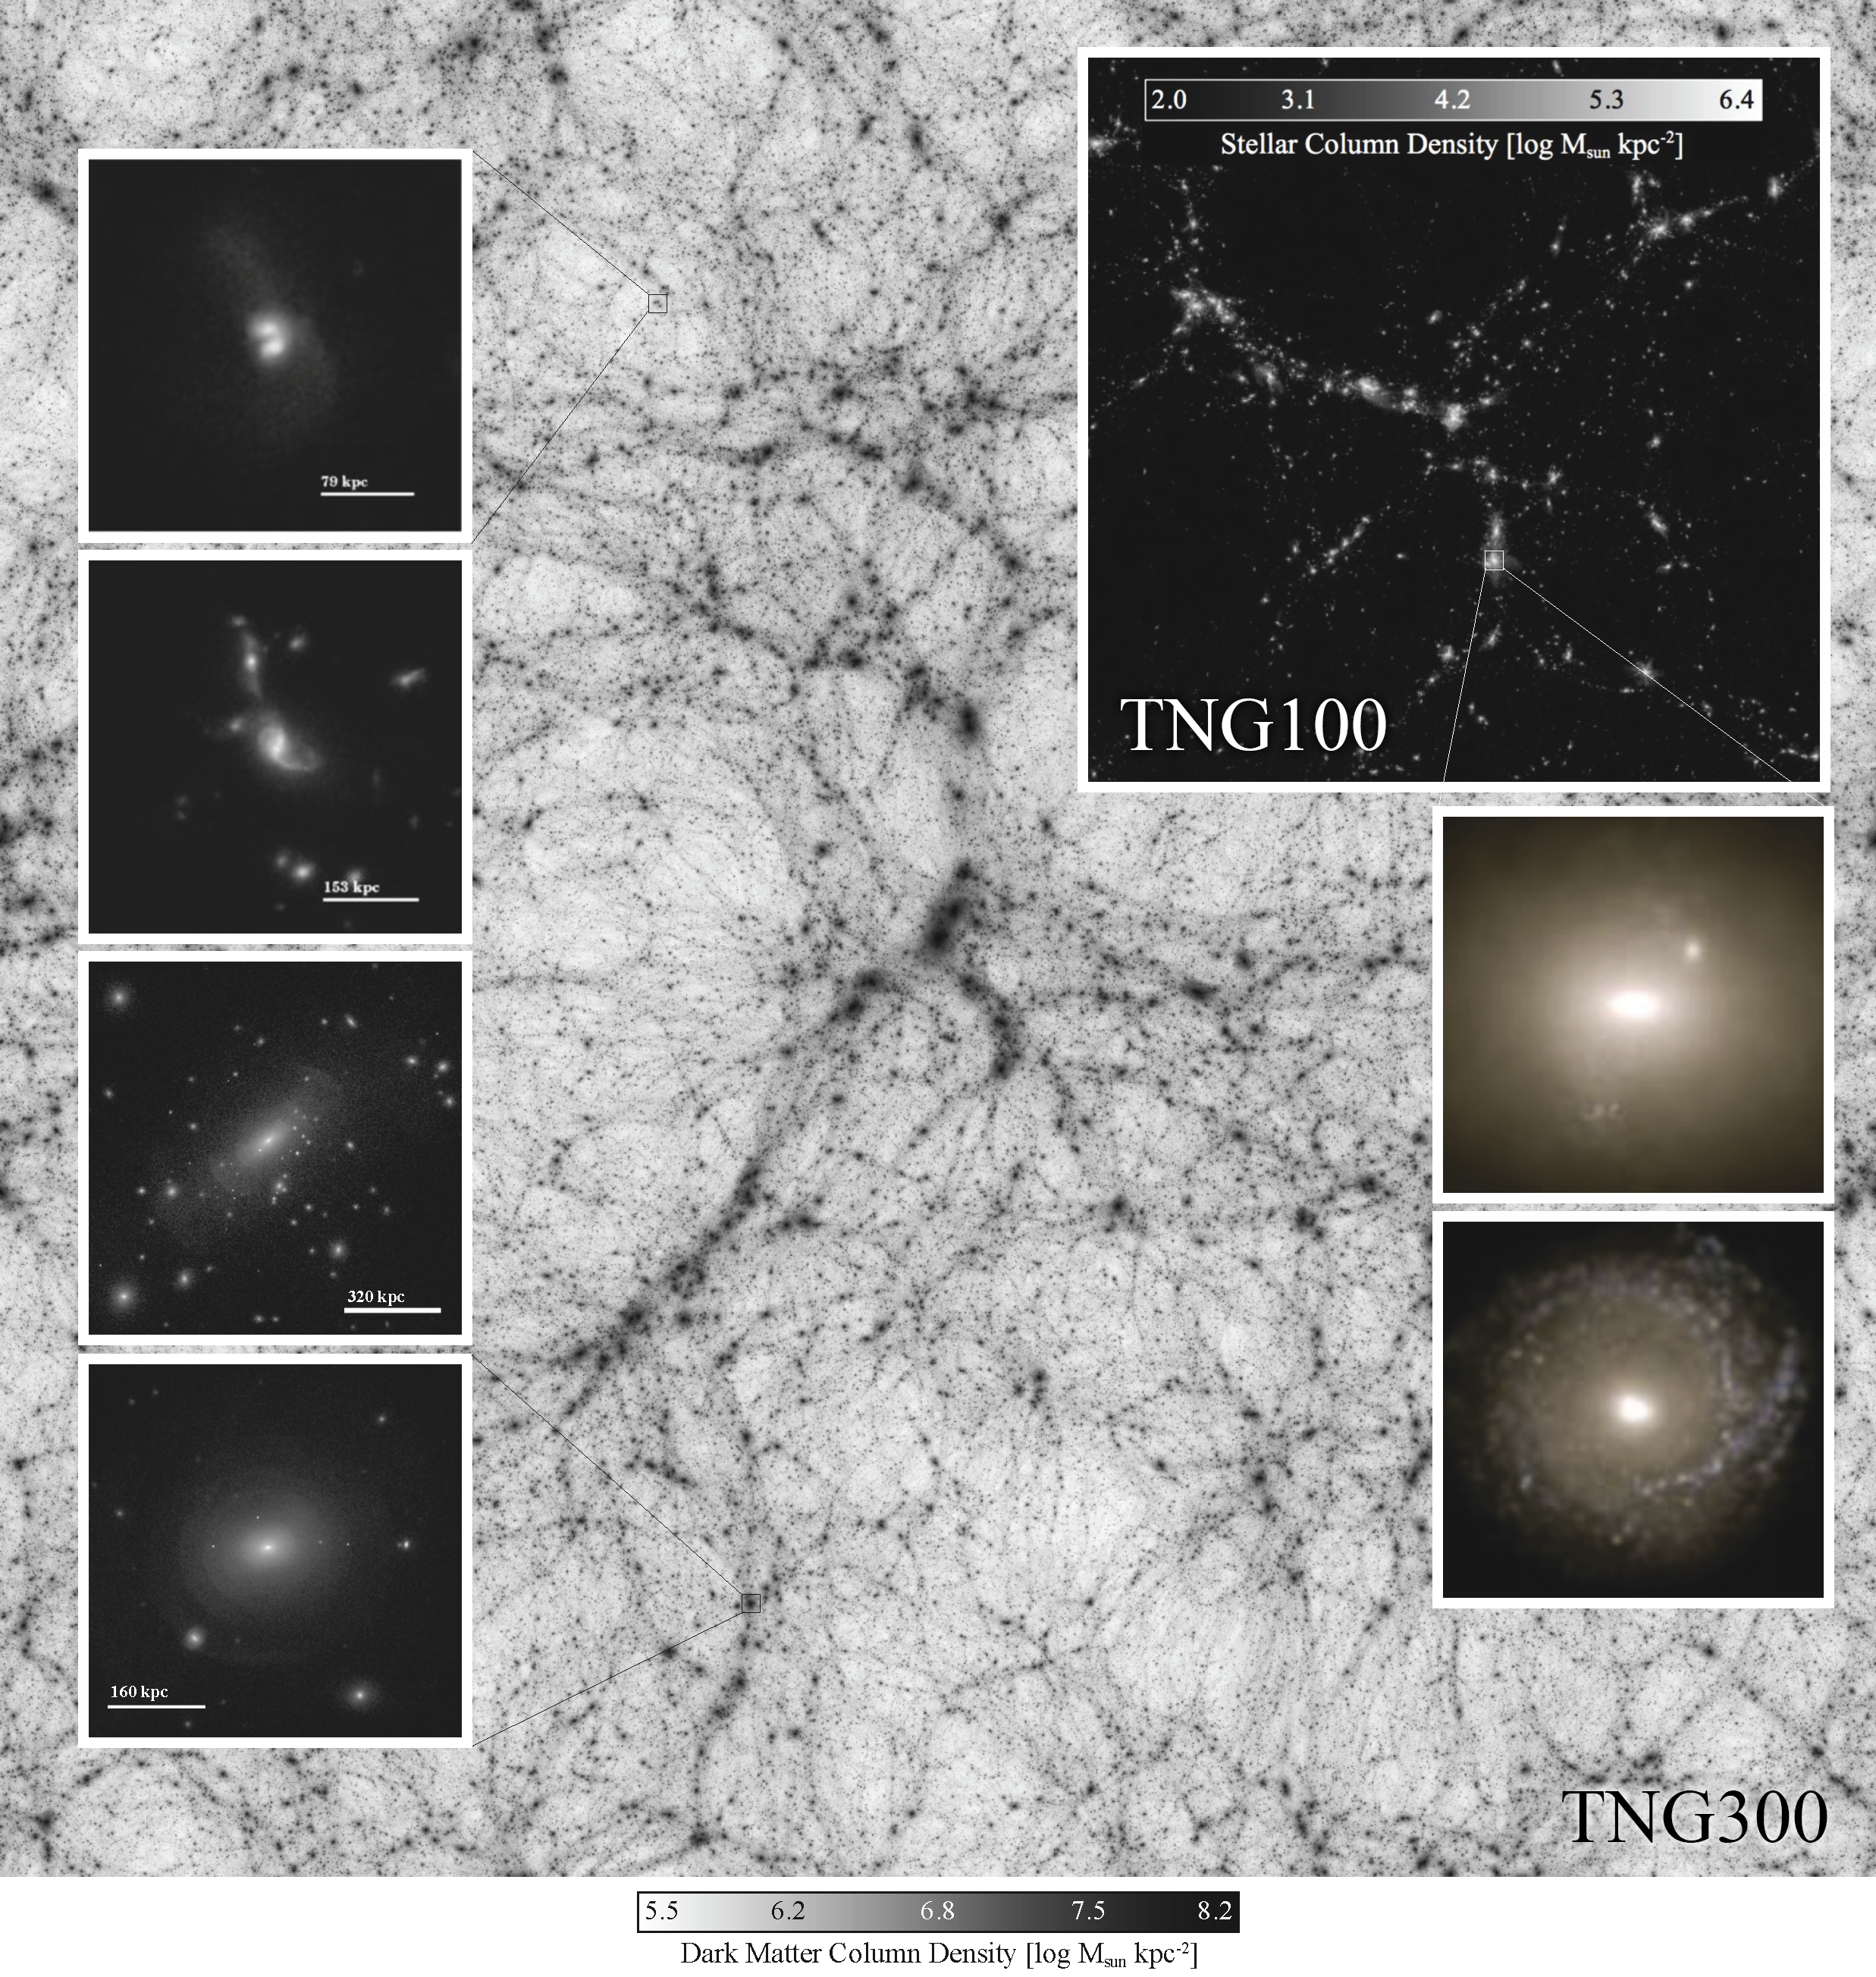
\includegraphics[width=0.9\textwidth]{images/TNG.png}
    \caption{A composite image that illustrates the two simulations TNG100 and TNG300. In the background is the dark matter distribution for the whole TNG300 volume. In the upper right is the stellar mass distribution across the entire TNG100 volume. The panels on the left show galaxy-galaxy interactions, while the panels on the right show the stellar light projections of two $z=0$ galaxies. Credit: TNG Collaboration}.
    \label{tng_illustration}
\end{figure}

\begin{table}
\begin{center}
\caption{The simulation details for the three main TNG simulations. $N_{DM}$ is the amount of dark matter particles. $m_{DM}$ and $m_{baryon}$ is the mass of the dark matter and baryonic particles, respectively.}
 \label{TNG}
\begin{tabular}{ l| c c c c c } 
 \hline
 \hline
   &  Volume [$Mpc^3$] & $N_{DM}$ & $m_{DM}$ [$M_{\odot}$] & $m_{baryon}$ [$M_{\odot}$] \\
 \hline
 TNG50 & $51.7^3$ & $2163^3$ & $4.5 \times 10^5 $ & $8.5 \times 10^4 $ \\ 
 TNG100 & $110.7^3$ & $1820^3$ & $7.5 \times 10^6 $ & $1.4 \times 10^6 $  \\ 
 TNG300 & $302.6^3$ & $2500^3$ & $5.9 \times 10^7 $ & $1.1 \times 10^7 $  \\ 
 \hline 
 \end{tabular}
\end{center}
\end{table}

\subsubsection{Data products}
All the Illustris-TNG data is publically available online at the TNG webpage\footnote{https://www.tng-project.org/data/}. The data products that are available for each simulation are snapshots, group catalogs, and merger trees as well as some supplementary data sets. There are five different particle types in the simulations, and each has its properties stored as particle fields. These fields include information like position, kinematic data, and chemical composition. For each different run of the simulation, 100 snapshots are created, which are taken at specific redshifts. They include all the particles in the whole volume of the simulation, with 20 of them including all the fields for each particle as well.

The group catalogs provide a convenient way to quickly access already calculated properties of the different halos and subhalos instead of dealing with all the particles in a snapshot. This saves a lot of time and effort but gives the user less control over what can be analyzed. There is one group catalog for each snapshot, and this includes two types of objects, Friends-of-Friends (FoF) and SUBFIND. The FoF catalog contains all the halos, and the SUBFIND catalog contains all the subhalos and their associated galaxy (if there is any) for each halo. Each subhalo has a parent halo, and the largest subhalo in each halo is the central subhalo. The merger trees data products contain the merger history of each subhalo.

This project makes use of the group catalogs and particles for the $z = 0$ snapshot.

\subsubsection{Sample reduction}

The TNG documentation recommends filtering out all subhalos that are flagged with the $SubhaloFlag$ field, and so these were cut from the data. They are most probably subhalos of non-cosmological origin, and so should not be considered real galaxies.

For this project, only the central galaxies in each halo are selected. The FoF catalog contains the index for the largest subhalo in each halo, so combining this information with the SUBFIND catalog allows one to create a subset of the data that contains only the central galaxies.

Only galaxies with stellar mass greater than $10^{9.5} M_{\odot}$ are used, which corresponds to about 4500 stellar particles.

\subsection{Galaxy sizes}
When observing galaxies with telescopes, there is always the problem of contamination of the measurements by surrounding sources as well as background radiation. As such, when the images are processed, aperture sizes have to be chosen with care for each identified galaxy. A larger aperture will be sure to contain most of the light from the galaxy but might overshoot by including surrounding light as well. However, choosing a too small aperture will result in lost data, and as such a smaller apparent galaxy. Usually a circular or elliptical aperture with a calculated radius to balance these two issues is chosen.

In simulations, we are not limited by hardware, attenuation, and background light. A cut-off point still needs to be determined. SUBFIND does this for the dark matter part of the simulation, separating out subhalos from larger halos. The galaxy properties of that subhalo are then calculated using all the stellar and gas particles in the subhalo and saved in the group catalog. 


When comparing simulation data to observational data, there are many ways to emulate the finite size of observed galaxies. Calculating luminosities and selecting a cut-off point at the faint end, using a spherical volume with a radius that is a multiple of their particular effective radius, or a fraction of the virial radius of the parent subhalo are some of the most commonly employed methods. For this work, the galaxy size is chosen to be a spherical volume with a radius ($R_{gal}$) equal to 15 \% of the subhalo's virial radius.

\subsection{Galaxy properties}

\subsubsection{Magnitude and colors}

The absolute magnitude ($\mathcal{M}$) is a measure of the total luminosity ($L$) of the galaxy such that $\mathcal{M} = -2.5 \log(L/L_\odot) + \mathcal{M}_\odot$, where $L_\odot$ is the solar luminosity and $\mathcal{M}_\odot$ is the solar magnitude.

For the SUBHALO group catalog, the \texttt{SubhaloStellarPhotometrics} field gives the magnitudes based on the summed up luminosities of all the stellar particles in the Subhalo. Our luminosities are determined by summing the luminosities within $R_{gal}$. Eight bands are available, but here only the g- and i-band are used. 

The g-i colors are calculated by simply subtracting the i-band magnitude from the g-band magnitude.

\subsubsection{Masses}

In SUBFIND, masses for each particle type are calculated by summing up all the masses of that particle type belonging to the halo. Values for the mass within the half-mass radius, two times the half-mass radius and the radius at which the maximum rotational velocity is found are also available.

The stellar masses of the galaxies studied using the particles are the summed up masses of all stellar particles within $R_{gal}$.

\subsubsection{Size}
For the group catalog, the \texttt{SubhaloHalfmassRadStellar} field has been used as the effective radius. The half-mass radius is the radius of a spherical volume within which half the stellar mass is found. It is the 3D half-mass radius ($R_e$), as it is not a projected quantity.

The half-mass radii of the galaxies calculated using the particles are calculated using the same method, but with the total stellar mass calculated within $R_{gal}$.

\subsubsection{Velocities}

Galaxy velocities are usually given by the velocity dispersion and rotational velocity for early and late-type galaxies, respectively. This is because of the difference in the shape of the two galaxy types. It makes more sense to talk about velocity dispersion in a spheroidal pressure-dominated system and rotational velocity in a rotating disk.

In SUBFIND, the field \texttt{SubhaloVMax} gives the maximum value for the spherically averaged rotation curve of a given galaxy. As the rotational curves are nearly flat for large enough radii, it should not be very important at which specific radius the observational rotational velocity is measured, as long as it is in the flat part of the curve. For observational data, a common practice is to look at the rotational velocities of stars in the outer part of the galaxy. To compare with SUBFIND's \texttt{SubhaloVMax}, the rotational velocity at a radius of $2.2 \times R_e$ was calculated for all galaxies.


In observations, the only velocities of the components of a galaxy we can measure are the line-of-sight velocities. These are calculated using the observed Doppler shift in the galactic spectrum. The velocity dispersion of a galaxy is then defined as the standard deviation of the line-of sight velocities.

\begin{equation} \label{standard_dev}
    \sigma^{2} = \frac{1}{N} \sum_{n=1}^{N} (V_{i} - \overline{V})^2
\end{equation}

If the velocity dispersion tends to fall off at larger radii, and the galaxy has an ellipsoid shape, the angle at which the galaxy is viewed will affect the observed velocity dispersion. To compensate for this when comparing simulations to observations, velocity dispersions in simulations may be calculated in three different projections of the galaxy and averaged over these. 

\begin{equation} \label{sigma1}
    \sigma^{2} = \frac{1}{3}(\sigma_x^2 + \sigma_y^2 + \sigma_z^2)
\end{equation}

In this work the velocity dispersion was calculated within the projected half-mass radius in each projection.

In SUBFIND, the velocity dispersion is simply calculated as the velocity dispersion of all the particles over the entire subhalo.


\subsection{Galaxy morphology classifications}

An important factor in many studies of galaxy formation and evolution is looking at the properties of the two morphological types of galaxies. As a visual classification method is intensively time-consuming, other methods have been devised for identifying early and late-type galaxies in simulations. In many studies, several of these classification criteria are used in conjunction.

\subsubsection{Gas fraction}
As early-type galaxies have much less cold gas than late-type galaxies, a simple cut in the galaxy population based on the gas fraction will be effective at roughly separating the two types. TNG doesn't differentiate between cold and hot gas, so it is important to consider the physical volume where the gas fraction is calculated. A large volume will inevitably contain more hot gas and potentially allow for early-type galaxies to be considered as late types. Late-type galaxies also have a wide range of gas fractions. The most massive spiral galaxies can contain as little as 5\% gas, while low-mass disks can contain up to 80\% \parencite{Mo2010}. In \textcite{Ferrero2020} galaxies with less than 10\% gas were considered for early types, while those with more were potential candidates for late-type classifications.

\subsubsection{Star formation rate}
Another way of separating galaxies into the early and late-type categories is by using the specific star formation rate (sSFR). The sSFR of a galaxy is the galaxy's star formation rate divided by the stellar mass content of the galaxy. In this case, the galaxies are tagged as ``quenched'' or ``main-sequence'', where quenched galaxies have little to no star formation, while main-sequence galaxies have a significant amount of star formation. More formally, they are separated by how far from the ridge of the star-formation main-sequence they are found (//cite). In \textcite{Genel2017} the ridge of the main-sequence is defined as the mean of the sSFR for galaxies with mass $10^{9} M_{\odot} < M_* < 10^{10.5} M_{\odot}$, and takes a value of $\log (sSFR[Gyr^{-1}]) = -0.94$ for $z=0$. Galaxies are then considered `main-sequence' if their sSFR are within 0.5 dex of this value. ``Quenched'' galaxies are defined as those with sSFR at least 1 dex below the ridge.

\subsubsection{Rotational kinetic energy}
A common way of estimating a galaxy's ``diskyness'' is to use the rotational-to-total-kinetic-energy parameter $\kappa_{rot}$. 
\begin{equation}
    \kappa_{rot} = \frac{K_{rot}}{K} = \frac{\sum_{i=1}^{N} m_i (j_{z, i}/R_i)^2}{\sum_{i=1}^{N} m_i v_i^2},
\end{equation}
where $j_{z, i}$ is the z-component of the specific angular momentum ($\vec{j} = \vec{r} \times \vec{v}$), $m_i$ is the mass, and $R_i$ is the projected radius of stellar particle $i$ in the xy-plane. 
This value indicates how much of the kinetic energy of the galaxy is invested in the ordered rotation about its axis. To calculate $\kappa_{rot}$, the axis of rotation must first be found. The galaxy is then rotated such that the z-axis of the galaxy's coordinate system is pointed in the direction of the axis of rotation, and $\kappa_{rot}$ is calculated.
For a perfect disk galaxy that is totally rotationally supported $\kappa_{rot} = 1$, while for a totally pressure supported system, $\kappa_{rot}$ would approach zero. In \textcite{Sales2012}, galaxies were classified as early type if they had $\kappa_{rot} < 0.5$ and late type for $\kappa_{rot} > 0.7$. This leads to a significant amount of ``intermediate types'', but other works have simply made use of a single cut at $\kappa_{rot} = 0.6$.